% p38

\section*{Solución propuesta}

\subsection*{1. Identificación del cliente y el servidor}
La solución constará de las siguientes partes:

\begin{itemize}
    \item \textbf{Servidor:} Computador Central (\texttt{CC})
    \item \textbf{Cliente $n$:} Computador del cajero $n$ (\texttt{Cn})
\end{itemize}

Por lo tanto, la arquitectura general de la solución es la siguiente:

\begin{figure}[h]
    \centering
    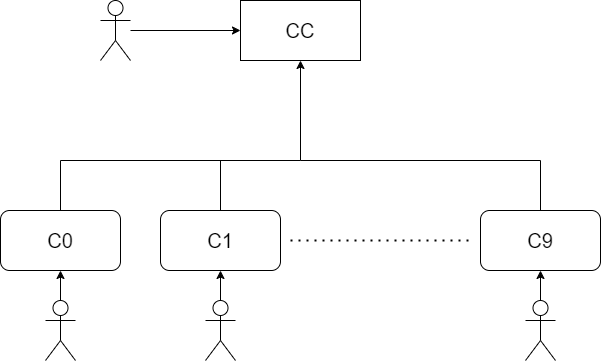
\includegraphics[width=0.6\textwidth]{img/arquitecture.png}
\end{figure}


\subsection*{2. Operaciones y secuencia de intercambio de mensajes}
El sistema contará con cuatro operaciones, con sus consiguientes secuencias de intercambio de mensajes:

\begin{itemize}
    \item \textbf{Apertura:} Cuando el cajero abre la caja.
    \begin{enumerate}
        \item \texttt{Cn} $\rightarrow$ \texttt{CC}: Datos de la caja, hora actual
        \item \texttt{CC} $\rightarrow$ \texttt{Cn}: 
        \begin{itemize}
            \item \texttt{OK} en caso de que todo haya ido bien.
            \item \texttt{KO} en caso de error (la caja ya está activa, la hora es incorrecta, etc.).
        \end{itemize}
    \end{enumerate}

    \item \textbf{Venta:} Cuando se produce una venta en el cajero.
    \begin{enumerate}
        \item \texttt{Cn} $\rightarrow$ \texttt{CC}: Datos de la caja, hora actual, total de la venta, artículos vendidos
        \item \texttt{CC} $\rightarrow$ \texttt{Cn}: 
        \begin{itemize}
            \item \texttt{OK} en caso de que todo haya ido bien.
            \item \texttt{KO} en caso de error (el total no coincide con la suma de los precios de los artículos, la hora es incorrecta, etc.).
        \end{itemize}
    \end{enumerate}
    
    \item \textbf{Cierre:} Cuando el cajero cierra la caja.
    \begin{enumerate}
        \item \texttt{Cn} $\rightarrow$ \texttt{CC}: Datos de la caja, hora actual, tiempo total, facturación total, artículos vendidos
        \item \texttt{CC} $\rightarrow$ \texttt{Cn}: 
        \begin{itemize}
            \item \texttt{OK} en caso de que todo haya ido bien.
            \item \texttt{KO} en caso de error (la caja ya está cerrada, la hora es incorrecta, el tiempo total no coincide con el registro, etc.).
        \end{itemize}
    \end{enumerate}
    
    \item \textbf{Monitorización:} Consulta de estado de una caja.
    \begin{enumerate}
        \item \texttt{CC} $\rightarrow$ \texttt{Cn}: Datos de la caja, hora actual
        \item \texttt{Cn} $\rightarrow$ \texttt{CC}: 
        \begin{itemize}
            \item En caso de que todo haya ido bien:
            \begin{enumerate}
                \item \texttt{OK}
                \item Datos de la caja, hora actual, tiempo total, estado, facturación total, artículos vendidos.
            \end{enumerate}
            \item \texttt{KO} en caso de error (hora incorrecta, identificador incorrecto, etc.).
        \end{itemize}
    \end{enumerate}
\end{itemize}

Nótese que en todos los mensajes el código de operación va incluído.

\subsection*{3. Protocolo}
\begin{itemize}
    \item Se usarán sockets TCP, dado que verifica que los paquetes llegan al destino, y eso es importante en esta aplicación.
    \item Se usará una conexión por peticion, ya que los intercambios de mensajes son cortos e infrecuentes, y permite ahorrar recursos.
\end{itemize}



\subsection*{4. Formato de los mensajes}

Partiendo del esquema general del punto 2, se especifica la estructura de los mensajes:

\begin{itemize}
    \item \textbf{Apertura:} Cuando el cajero abre la caja.
    \begin{enumerate}
        \item \texttt{Cn} $\rightarrow$ \texttt{CC}: \texttt{\{opcode (open), id, num-caja, hora\}}
        \item \texttt{CC} $\rightarrow$ \texttt{Cn}: 
        \begin{itemize}
            \item \texttt{OK} en caso de que todo haya ido bien.
            \item \texttt{KO} en caso de error (la caja ya está activa, la hora es incorrecta, etc.).
        \end{itemize}
    \end{enumerate}

    \item \textbf{Venta:} Cuando se produce una venta en el cajero.
    \begin{enumerate}
        \item \texttt{Cn} $\rightarrow$ \texttt{CC}: \texttt{\{opcode (sell), id, num-caja, hora, importe-total, num-artículos,\\
        id-artículo-0, precio-artículo-0, [...]\}}
        \item \texttt{CC} $\rightarrow$ \texttt{Cn}: 
        \begin{itemize}
            \item \texttt{OK} en caso de que todo haya ido bien.
            \item \texttt{KO} en caso de error (el total no coincide con la suma de los precios de los artículos, la hora es incorrecta, etc.).
        \end{itemize}
    \end{enumerate}
    
    \item \textbf{Cierre:} Cuando el cajero cierra la caja.
    \begin{enumerate}
        \item \texttt{Cn} $\rightarrow$ \texttt{CC}: \texttt{\{opcode (close), id, num-caja, hora, importe-total,\\
        tiempo-total, num-artículos\}}
        \item \texttt{CC} $\rightarrow$ \texttt{Cn}: 
        \begin{itemize}
            \item \texttt{OK} en caso de que todo haya ido bien.
            \item \texttt{KO} en caso de error (la caja ya está cerrada, la hora es incorrecta, el tiempo total no coincide con el registro, etc.).
        \end{itemize}
    \end{enumerate}
    
    \item \textbf{Monitorización:} Consulta de estado de una caja.
    \begin{enumerate}
        \item \texttt{CC} $\rightarrow$ \texttt{Cn}: \texttt{\{opcode (status), id, num-caja, hora\}}
        \item \texttt{Cn} $\rightarrow$ \texttt{CC}: 
        \begin{itemize}
            \item En caso de que todo haya ido bien:
            \begin{enumerate}
                \item \texttt{OK}
                \item \texttt{\{id, num-caja, hora, estado (abierta|cerrada), importe-total,\\
                tiempo-total, num-artículos\}}.
            \end{enumerate}
            \item \texttt{KO} en caso de error (hora incorrecta, identificador incorrecto, etc.).
        \end{itemize}
    \end{enumerate}
\end{itemize}

Los diferentes parámetros cuentan con el siguiente formato:
\begin{itemize}
    \item \textbf{\texttt{opcode}:} Array de un caracter numérico que identifica la operación.\\
    Dependiendo de la operación:
    \begin{itemize}
        \item \textbf{\texttt{open}:} \texttt{0}
        \item \textbf{\texttt{sell}:} \texttt{1}
        \item \textbf{\texttt{close}:} \texttt{2}
        \item \textbf{\texttt{status}:} \texttt{3}
    \end{itemize}
    \item \textbf{\texttt{id}:} Array de nueve caracteres que identifica al empleado.
    \item \textbf{\texttt{num-caja}:} Array de dos caracteres que identifica la caja, e.g. \texttt{C2}.
    \item \textbf{\texttt{hora}:} Array de once caracteres con la hora en formato \texttt{HH:MM:SS:ns}.
    \item \textbf{\texttt{importe-total}:} Array de diez caracteres con el importe total de una compra o facturación, en formato \texttt{XXXXXX,XX€}.
    \item \textbf{\texttt{num-artículos}:} Array de tres caracteres numéricos que indica el número de artículos vendidos.
    \item \textbf{\texttt{id-artículo-n}:} Array de seis caracteres que indica el id de un artículo \textit{n}.
    \item \textbf{\texttt{precio-artículo-n}:} Array de nueve caracteres con el precio de un artículo \textit{n}, en formato \texttt{XXXXX,XX€}.
    \item \textbf{\texttt{tiempo-total}:} Array de nueve caracteres que indica el número de minutos que la caja lleva abierta.
    \item \textbf{\texttt{estado}:} Array de un caracter numérico que indica el estado de la caja:
    \begin{itemize}
        \item \textbf{\texttt{abierta}:} \texttt{0}
        \item \textbf{\texttt{cerrada}:} \texttt{1}
    \end{itemize}
\end{itemize}

Todos los mensajes terminarán también con el caracter \texttt{\textbackslash{}0} para marcar el fin de la cadena.

\subsection*{5. Concurrencia}

El Computador Central acepta peticiones de las cajas en un hilo secundario, y por cada petición lanza un hilo para atenderlo, dado que se se usa una conexión por petición. Estos hilos acceden a una base de datos donde guardar y consultar la información, usando mecanismos de concurrencia para garantizar la exclusión y la coherencia en el acceso a los datos.\\
El hilo principal estará pendiente de atender al usuario del Computador Central para enviar las peticiones requeridas.\newline

Cada Cajero lanza un hilo secundario para atender las peticiones del Computador Central y responderlas, mientras que el hilo principal se encarga de enviar las peticiones requeridas al Computador Central.\\
Se procurará el acceso a una base de datos donde guardar y consultar la información, usando mecanismos de concurrencia para garantizar la exclusión y la coherencia en el acceso a los datos.


\subsection*{6. Nombrado}

Por motivos de seguridad, y asumiendo que en principio el número de cajas se mantendrá, se utilizará un direccionamiento estático.\\
Las IPs de los equipos se conocen, y pertenecen a la misma red local, por lo que habrá que configurar manualmente los \textit{hostname} de las máquinas.\newline

Cada cajero sólo conocerá la IP del Computador Central, mientras que el CC conocerá las IPs de todas las cajas.


\subsection*{7. Diseño final}

Debido al diseño de concurrencia de las cajas, el CC necesitará saber el puerto al que enviar a la caja las peticiones. Por lo tanto, se deberá modificar el mensaje de apertura, quedando lo siguiente:
\begin{enumerate}
    \item \texttt{Cn} $\rightarrow$ \texttt{CC}: \texttt{\{opcode (open), id, num-caja, hora, puerto\}}
    \item \texttt{CC} $\rightarrow$ \texttt{Cn}: 
    \begin{itemize}
        \item \texttt{OK} en caso de que todo haya ido bien.
        \item \texttt{KO} en caso de error (la caja ya está activa, la hora es incorrecta, etc.).
    \end{itemize}
\end{enumerate}

Donde \texttt{puerto} es un array de cuatro caracteres numéricos que indica el puerto de escucha del cajero.